% (find-LATEX "2020-2-C3-P1.tex")
% (defun c () (interactive) (find-LATEXsh "lualatex -record 2020-2-C3-P1.tex" :end))
% (defun C () (interactive) (find-LATEXsh "lualatex 2020-2-C3-P1.tex" "Success!!!"))
% (defun D () (interactive) (find-pdf-page      "~/LATEX/2020-2-C3-P1.pdf"))
% (defun d () (interactive) (find-pdftools-page "~/LATEX/2020-2-C3-P1.pdf"))
% (defun e () (interactive) (find-LATEX "2020-2-C3-P1.tex"))
% (defun o () (interactive) (find-LATEX "2020-2-C3-P1.tex"))
% (defun u () (interactive) (find-latex-upload-links "2020-2-C3-P1"))
% (defun v () (interactive) (find-2a '(e) '(d)))
% (defun d0 () (interactive) (find-ebuffer "2020-2-C3-P1.pdf"))
% (defun cv () (interactive) (C) (ee-kill-this-buffer) (v) (g))
%          (code-eec-LATEX "2020-2-C3-P1")
% (find-pdf-page   "~/LATEX/2020-2-C3-P1.pdf")
% (find-sh0 "cp -v  ~/LATEX/2020-2-C3-P1.pdf /tmp/")
% (find-sh0 "cp -v  ~/LATEX/2020-2-C3-P1.pdf /tmp/pen/")
%     (find-xournalpp "/tmp/2020-2-C3-P1.pdf")
%   file:///home/edrx/LATEX/2020-2-C3-P1.pdf
%               file:///tmp/2020-2-C3-P1.pdf
%           file:///tmp/pen/2020-2-C3-P1.pdf
% http://angg.twu.net/LATEX/2020-2-C3-P1.pdf
% (find-LATEX "2019.mk")
% (find-CN-aula-links "2020-2-C3-P1" "3" "c3m202p1" "c3p1")
%
% Video:
% (find-ssr-links "c3m202p1" "2020-2-C3-P1")
% (code-video     "c3m202p1video" "$S/http/angg.twu.net/eev-videos/2020-2-C3-P1.mp4")
% (find-c3m202p1video "0:00")

% «.defs»		(to "defs")
% «.defs-T-and-B»	(to "defs-T-and-B")
% «.title»		(to "title")
% «.regras-e-dicas»	(to "regras-e-dicas")
% «.questao-1»		(to "questao-1")
% «.questao-2»		(to "questao-2")
% «.gabarito-1»		(to "gabarito-1")
% «.numerozinhos»	(to "numerozinhos")
% «.gabarito-2»		(to "gabarito-2")
%
% «.djvuize»	(to "djvuize")

\documentclass[oneside,12pt]{article}
\usepackage[colorlinks,citecolor=DarkRed,urlcolor=DarkRed]{hyperref} % (find-es "tex" "hyperref")
\usepackage{amsmath}
\usepackage{amsfonts}
\usepackage{amssymb}
\usepackage{pict2e}
\usepackage[x11names,svgnames]{xcolor} % (find-es "tex" "xcolor")
\usepackage{colorweb}                  % (find-es "tex" "colorweb")
%\usepackage{tikz}
%
% (find-dn6 "preamble6.lua" "preamble0")
%\usepackage{proof}   % For derivation trees ("%:" lines)
%\input diagxy        % For 2D diagrams ("%D" lines)
%\xyoption{curve}     % For the ".curve=" feature in 2D diagrams
%
\usepackage{edrx15}               % (find-LATEX "edrx15.sty")
\input edrxaccents.tex            % (find-LATEX "edrxaccents.tex")
\input edrxchars.tex              % (find-LATEX "edrxchars.tex")
\input edrxheadfoot.tex           % (find-LATEX "edrxheadfoot.tex")
\input edrxgac2.tex               % (find-LATEX "edrxgac2.tex")
\input 2017planar-has-defs.tex    % (find-LATEX "2017planar-has-defs.tex")
%
%\usepackage[backend=biber,
%   style=alphabetic]{biblatex}            % (find-es "tex" "biber")
%\addbibresource{catsem-slides.bib}        % (find-LATEX "catsem-slides.bib")
%
% (find-es "tex" "geometry")
\usepackage[a6paper, landscape,
            top=1.5cm, bottom=.25cm, left=1cm, right=1cm, includefoot
           ]{geometry}
%
\begin{document}

\catcode`\^^J=10
\directlua{dofile "dednat6load.lua"}  % (find-LATEX "dednat6load.lua")

%L dofile "edrxtikz.lua"  -- (find-LATEX "edrxtikz.lua")
%L dofile "edrxpict.lua"  -- (find-LATEX "edrxpict.lua")
\pu

% «defs»  (to ".defs")
% (find-LATEX "edrx15.sty" "colors-2019")
\long\def\ColorRed   #1{{\color{Red1}#1}}
\long\def\ColorViolet#1{{\color{MagentaVioletLight}#1}}
\long\def\ColorViolet#1{{\color{Violet!50!black}#1}}
\long\def\ColorGreen #1{{\color{SpringDarkHard}#1}}
\long\def\ColorGreen #1{{\color{SpringGreenDark}#1}}
\long\def\ColorGreen #1{{\color{SpringGreen4}#1}}
\long\def\ColorGray  #1{{\color{GrayLight}#1}}
\long\def\ColorGray  #1{{\color{black!30!white}#1}}
\long\def\ColorBrown #1{{\color{Brown}#1}}
\long\def\ColorBrown #1{{\color{brown}#1}}
\long\def\ColorOrange#1{{\color{orange}#1}}

\long\def\ColorShort #1{{\color{SpringGreen4}#1}}
\long\def\ColorLong  #1{{\color{Red1}#1}}

\def\frown{\ensuremath{{=}{(}}}
\def\True {\mathbf{V}}
\def\False{\mathbf{F}}
\def\Max  {\mathsf{max}}
\def\Min  {\mathsf{min}}
\def\D    {\displaystyle}

\long\def\ColorRed   #1{{\color{Red1}#1}}
\long\def\ColorViolet#1{{\color{MagentaVioletLight}#1}}
\long\def\ColorViolet#1{{\color{Violet!50!black}#1}}
\long\def\ColorGreen #1{{\color{SpringDarkHard}#1}}
\long\def\ColorGreen #1{{\color{SpringGreenDark}#1}}
\long\def\ColorGreen #1{{\color{SpringGreen4}#1}}
\long\def\ColorOrange#1{{\color{orange!90!black}#1}}
\long\def\ColorGray  #1{{\color{GrayLight}#1}}
\long\def\ColorGray  #1{{\color{black!30!white}#1}}

\def\drafturl{http://angg.twu.net/LATEX/2020-2-C3.pdf}
\def\drafturl{http://angg.twu.net/2020.2-C3.html}
\def\draftfooter{\tiny \href{\drafturl}{\jobname{}} \ColorBrown{\shorttoday{} \hours}}

% «defs-T-and-B»  (to ".defs-T-and-B")
% (c3m202p1p 6 "questao-2")
% (c3m202p1    "questao-2")
\def\T(Total: #1 pts){{\bf(Total: #1)}}
\def\T(Total: #1 pts){{\bf(Total: #1 pts)}}
\def\T(Total: #1 pts){\ColorRed{\bf(Total: #1 pts)}}
\def\B       (#1 pts){\ColorOrange{\bf(#1 pts)}}




%  _____ _ _   _                               
% |_   _(_) |_| | ___   _ __   __ _  __ _  ___ 
%   | | | | __| |/ _ \ | '_ \ / _` |/ _` |/ _ \
%   | | | | |_| |  __/ | |_) | (_| | (_| |  __/
%   |_| |_|\__|_|\___| | .__/ \__,_|\__, |\___|
%                      |_|          |___/      
%
% «title»  (to ".title")
% (c3m202p1p 1 "title")
% (c3m202p1    "title")

\thispagestyle{empty}

\begin{center}

\vspace*{1.2cm}

{\bf \Large Cálculo 3 - 2020.2}

\bsk

P1 (Primeira prova)

\bsk

Eduardo Ochs - RCN/PURO/UFF

\url{http://angg.twu.net/2020.2-C3.html}

\end{center}

\newpage

% «regras-e-dicas»  (to ".regras-e-dicas")
% (c3m202p1p 2 "regras-e-dicas")
% (c3m202p1    "regras-e-dicas")
% (c2m202p1p 2 "regras-e-dicas")
% (c2m202p1    "regras-e-dicas")

{\bf Regras e dicas}

As regras e dicas são as mesmas dos mini-testes:

\ssk

\url{http://angg.twu.net/LATEX/2020-2-C3-MT1.pdf}

\url{http://angg.twu.net/LATEX/2020-2-C3-MT2.pdf}

\ssk

exceto que a prova vai ser disponibilizada às 21:00 do dia

16/abril/2021 e deve ser entregue até as 21:30 do dia

17/abril/2021.

\newpage

% «questao-1»  (to ".questao-1")
% (c3m202p1p 3 "questao-1")
% (c3m202p1    "questao-1")

{\bf Questão 1.}

\T(Total: 7.5 pts)

\msk

Sejam:
%
$$\begin{array}{rcl}
    f(t) &=& \Min(\Max(0,t),3),     \\
  G(x,y) &=& \Min(x,y),             \\
  H(x,y) &=& f(\Min(x,y)).          \\
  S      &=& \setofxyzst{z=H(x,y)}, \\
  A(z)   &=& \setofxyst{H(x,y)=z},  \\
  B(x_0) &=& \setofst{(x,y,z)∈S}{x=x_0} \\
  C(y_0) &=& \setofst{(x,y,z)∈S}{y=y_0} \\
  D(z_0) &=& \setofst{(x,y,z)∈S}{z=z_0} \\
  \end{array}
$$

a) \B(0.5 pts) Faça o gráfico da função $f(t)$.

\newpage

{\bf Questão 1 (cont.)}


Faça o diagrama de numerozinhos para as funções:

b) \B(0.5 pts) $G(x,y)$,

c) \B(1.0 pts) $H(x,y)$;

use $x,y∈\{-1,0,1,2,3,4\}$.

\msk

d) \B(1.0 pts) Represente graficamente $A(1)$ e $A(2)$. 

e) \B(1.0 pts) Represente graficamente $A(0)$ e $A(3)$. 

Você pode fazer os itens d e e num gráfico só se quiser.

\newpage

{\bf Questão 1 (cont.)}

f) \B(3.5 pts) Represente graficamente num gráfico só, em 3D,

em perspectiva improvisada:

$B(-1), B(0), B(1), B(2), B(3), B(4),$

$C(-1), C(0), C(1), C(2), C(3), C(4)$.

\msk

Dica: isto é mais fácil com os eixos nesta posição:

% (find-latexscan-links "C3" "20210416_eixos")
% (find-xpdf-page "~/LATEX/2020-2-C3/20210416_eixos.pdf")
$$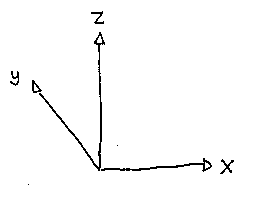
\includegraphics[height=3cm]{2020-2-C3/20210416_eixos.pdf}$$





\newpage

% «questao-2»  (to ".questao-2")
% (c3m202p1p 6 "questao-2")
% (c3m202p1    "questao-2")
% (c3m202taylor1p 1 "taylor-1")
% (c3m202taylor1    "taylor-1")

{\bf Questão 2.}

\T(Total: 3.0 pts)

\msk

Seja $f(x) = \arctan x$.

Sabemos que $f(1) = \frac{π}{4}$, $f'(1) = \frac12$, $f''(1) = -\frac12$, $f'''(1) = \frac12$.
 
Use isto para obter:

\msk

a) \B(1.5 pts) Uma aproximação de grau 3 para $f$

em torno do ponto 1.

\msk

b) \B(1.5 pts) Uma aproximação com 5 dígitos de precisão

para $f(1.1)$, fazendo as contas explicitamente.

Use $\fracπ4 ≈ 0.78450$.

% (/ pi 4)



\newpage

\thispagestyle{empty}

\begin{center}

\vspace*{2.0cm}

{\bf \Large Gabarito}

(incompleto)

\end{center}


\newpage

% «gabarito-1»  (to ".gabarito-1")
% (c3m202p1p 4 "gabarito-1")
% (c3m202p1    "gabarito-1")
% (find-es "dednat" "numerozinhos")

{\bf Questão 1: gabarito}

a) 
$\qquad
 f(x) \;\; = \;\;
 \vcenter{\hbox{%
 \unitlength=10pt
 \beginpicture(-2,-1)(5,4)
   \pictgrid%
   \pictpiecewise{(-2,0)--(0,0)--(3,3)--(5,3)
                  }%
   \pictaxes%
 \end{picture}%
 }}
$


% «numerozinhos»  (to ".numerozinhos")
% (find-es "dednat" "numerozinhos")
%
%L MixedPicture.__index.addnumerosaxes = function (mp, xmin, xmax, ymin, ymax)
%L     mp.lp:addt("\\Line(%s,0)(%s,0)", xmin-0.5, xmax+0.5)
%L     mp.lp:addt("\\Line(0,%s)(0,%s)", ymin-0.5, ymax+0.5)
%L     return mp
%L   end
%L MixedPicture.__index.addnumerozinhos = function (mp, xmin, xmax, ymin, ymax, f)
%L     for y=ymin,ymax do
%L       for x=xmin,xmax do
%L         mp:put(v(x,y), tostring(f(x,y)))
%L       end
%L     end
%L     return mp
%L   end
%L 
%L f = function (t) return min(max(0,t),3) end
%L G = function (x,y) return min(x,y) end
%L H = function (x,y) return f(min(x,y)) end
%L
%L mp = MixedPicture.new({zdef="G", scale="20pt", meta=""})
%L mp:addnumerosaxes (-1,4, -1,4)
%L mp:addnumerozinhos(-1,4, -1,4, G)
%L mp:output()
%L
%L mp = MixedPicture.new({zdef="H", scale="20pt", meta=""})
%L mp:addnumerosaxes (-1,4, -1,4)
%L mp:addnumerozinhos(-1,4, -1,4, H)
%L mp:output()
\pu

\msk

b) $G(x,y) = \scalebox{0.5}{$ \zha{G} $}$
%
\quad
%
c) $H(x,y) = \scalebox{0.5}{$ \zha{H} $}$

\msk

d,e)
\qquad
%
% (find-latexscan-links "C3" "20210430_C3_P1_gab_1d_1e")
% (find-xpdf-page "~/LATEX/2020-2-C3/20210430_C3_P1_gab_1d_1e.pdf")
$\myvcenter{
 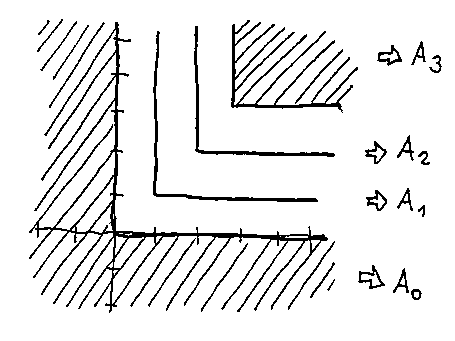
\includegraphics[height=2.5cm]{2020-2-C3/20210430_C3_P1_gab_1d_1e.pdf}
 }
$

\newpage

1f)
% (find-latexscan-links "C3" "20210430_C3_P1_gab_1f")
% (find-xpdf-page "~/LATEX/2020-2-C3/20210430_C3_P1_gab_1f.pdf")
$\myvcenter{
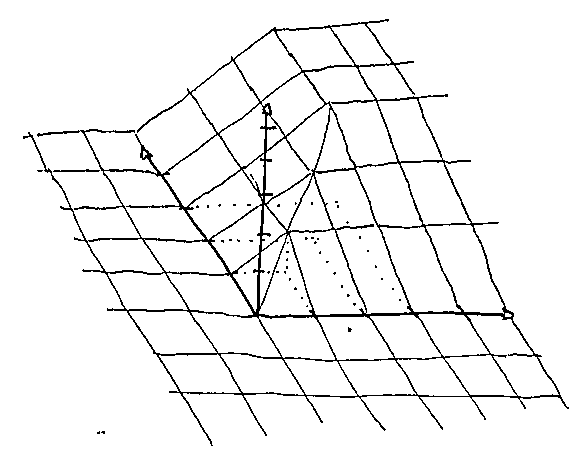
\includegraphics[height=8cm]{2020-2-C3/20210430_C3_P1_gab_1f.pdf}
 }
$


% (find-LATEX "2020-2-C2-ids-trigs.tex" "div-polis")


\newpage

% «gabarito-2»  (to ".gabarito-2")
% (c3m202p1p 4 "gabarito-2")
% (c3m202p1    "gabarito-2")

{\bf Questão 2: gabarito}

Sabemos que $f(1) = \frac{π}{4}$, $f'(1) = \frac12$, $f''(1) = -\frac12$, $f'''(1) = \frac12$.

Então:
%
$$\begin{array}{rcl}
  f(1+t) &≈& f(1) + f'(1)·t + \frac{f''(1)}{2}·t^2 + \frac{f''(1)}{6}·t^3 \\
         &=& \frac{π}{4} + \frac{1}{2}·t - \frac{1}{4}·t^2 + \frac{1}{12}·t^3 \\
  f(1.1) &≈& \frac{π}{4} + \frac{1}{20}  - \frac{1}{400}   + \frac{1}{12000} \\
         &≈& 0.78450 + 0.05  - 0.0025   + 0.00008 \\
         &=& 0.83208 \\
  \end{array}
$$

% (+ 0.78450 0.05  0.0025 0.00008)
% (+ 0.78450 0.05 -0.0025 0.00008)
% (atan 1.1)

Segundo o computador $\arctan 1.1 ≈ 0.83298$.

Deve ter uns erros de conta aí em cima...

Vou consertar depois.



%\printbibliography

\GenericWarning{Success:}{Success!!!}  % Used by `M-x cv'

\end{document}

%  ____  _             _         
% |  _ \(_)_   ___   _(_)_______ 
% | | | | \ \ / / | | | |_  / _ \
% | |_| | |\ V /| |_| | |/ /  __/
% |____// | \_/  \__,_|_/___\___|
%     |__/                       
%
% «djvuize»  (to ".djvuize")
% (find-LATEXgrep "grep --color -nH --null -e djvuize 2020-1*.tex")

 (eepitch-shell)
 (eepitch-kill)
 (eepitch-shell)
# (find-fline "~/2020.2-C3/")
# (find-fline "~/LATEX/2020-2-C3/")
# (find-fline "~/bin/djvuize")

cd /tmp/
for i in *.jpg; do echo f $(basename $i .jpg); done

f () { rm -fv $1.png $1.pdf; djvuize $1.pdf }
f () { rm -fv $1.png $1.pdf; djvuize WHITEBOARDOPTS="-m 1.0" $1.pdf; xpdf $1.pdf }
f () { rm -fv $1.png $1.pdf; djvuize WHITEBOARDOPTS="-m 0.5" $1.pdf; xpdf $1.pdf }
f () { rm -fv $1.png $1.pdf; djvuize WHITEBOARDOPTS="-m 0.25" $1.pdf; xpdf $1.pdf }
f () { cp -fv $1.png $1.pdf       ~/2020.2-C3/
       cp -fv        $1.pdf ~/LATEX/2020-2-C3/
       cat <<%%%
% (find-latexscan-links "C3" "$1")
%%%
}

f 20210430_C3_P1_gab_1d_1e
f 20210430_C3_P1_gab_1f

f 20210427_C3_gab

f 20210416_eixos



%  __  __       _        
% |  \/  | __ _| | _____ 
% | |\/| |/ _` | |/ / _ \
% | |  | | (_| |   <  __/
% |_|  |_|\__,_|_|\_\___|
%                        
% <make>

 (eepitch-shell)
 (eepitch-kill)
 (eepitch-shell)
# (find-LATEXfile "2019planar-has-1.mk")
make -f 2019.mk STEM=2020-2-C3-P1 veryclean
make -f 2019.mk STEM=2020-2-C3-P1 pdf

% Local Variables:
% coding: utf-8-unix
% ee-tla: "c3m202p1"
% End:
